\documentclass[11pt,a4paper]{article}

% --- Essential Packages ---
\usepackage[utf8]{inputenc}
\usepackage[T1]{fontenc}
\usepackage{lmodern}
\usepackage[margin=1in]{geometry}
\usepackage{amsmath,amssymb}
\usepackage{graphicx}
\usepackage{booktabs}
\usepackage{tabularx}
\usepackage{multirow}
\usepackage{xcolor}
\usepackage{microtype}
\usepackage{authblk}
\usepackage{caption}
\usepackage{float}
\usepackage{url}
\usepackage[round,authoryear]{natbib}
\usepackage[colorlinks=true,
            linkcolor=blue!70!black,
            citecolor=teal!70!black,
            urlcolor=blue!70!black]{hyperref}
\usepackage[capitalize,noabbrev]{cleveref}

% --- Document Metadata ---
\title{\textbf{Mining the Extraterrestrial Seedling Microbiome: Meta-transcriptomic Discovery of Endophytic and Commensal Communities in Spaceflight \textit{Arabidopsis thaliana}}}

\author[1,*]{Richard J. Barker}
\author[1]{Zerrin Sogutmaz Ozgen}
\author[2]{Sarah E. Wyatt}
\author[3]{Simon Gilroy}
\author[1,4]{NASA GeneLab Plant Analysis Working Group (AWG)}

\affil[1]{AstroBotany Laboratory and Artificial Intelligence Research Initiative (AIRI), Madison, WI, USA}
\affil[2]{Department of Environmental and Plant Biology, Ohio University, Athens, OH, USA}
\affil[3]{Department of Botany, University of Wisconsin--Madison, Madison, WI, USA}
\affil[4]{NASA Ames Research Center, Space Biosciences Division, Moffett Field, CA, USA}
\affil[*]{Corresponding author: \texttt{richard.barker@nasa.gov}}

\date{\today}

\begin{document}

\maketitle

% --- Abstract ---
\begin{abstract}
\textbf{Background:} Spaceflight exposes biological systems to the synergistic stresses of microgravity, cosmic ionizing radiation, and sealed atmospheric confinement. While the transcriptional responses of model plants like \textit{Arabidopsis thaliana} have been comprehensively cataloged in the NASA Open Science Data Repository (OSDR), the endophytic and epiphytic microbiomes associated with these seedlings have remained virtually unexplored in archival transcriptomic datasets. Because standard eukaryotic RNA sequencing protocols capture both host and microbial polyadenylated or co-extracted transcripts, mining unmapped non-host reads provides a powerful window into plant-microbiome dynamics in extraterrestrial environments.

\textbf{Methods:} Here, we present a systematic meta-transcriptomic extraction and taxonomic profiling pipeline applied across six OSDR spaceflight accessions (OSD-37, OSD-38, OSD-120, OSD-217, OSD-321, and OSD-522) encompassing multiple hardware systems (BRIC-19, BRIC-20, APEX-03-2, BRIC-PDF) and genetic backgrounds (Columbia-0, Wassilewskija-2, Landsberg \textit{erecta}-0, and Cape Verde Islands-0). Following host read subtraction against the \textit{A. thaliana} TAIR10 reference genome, remaining microbial sequences were profiled using MetaPhlAn4, Bowtie2, and Krona interactive visualization. Taxonomic intersections across flight and ground controls were assessed through UpSetR and hierarchical correlation analyses, and annotated using The Microbe Directory.

\textbf{Results:} We observed distinct microbial communities segregated between intrinsic seed-borne endophytes and extrinsic hardware- or human-associated commensals. \textit{Ralstonia pickettii} exhibited pervasive dominance across OSD-37 ecotypes, reaching 100\% relative abundance in Cvi-0 samples. In OSD-38, we uncovered the presence of \textit{Weizmannia ginsengihumi}, a beneficial plant-growth-promoting Firmicute previously unrecorded in orbital seedling habitats. Furthermore, common skin and environmental commensals including \textit{Cutibacterium acnes}, \textit{Malassezia restricta}, and \textit{Escherichia coli} were systematically identified, reflecting microbial exchange between crew-handled hardware and plant growth substrates. Interestingly, comparison of whole seedlings (OSD-37, 38) against dissected root tips (OSD-120) confirmed that endophytic colonization is strongly tissue-dependent, with root tips displaying near-complete depletion of bacterial transcripts.

\textbf{Conclusions:} These findings demonstrate that plant-associated microbiomes persist in closed spaceflight hardware and undergo community shifts that mirror both host developmental state and chamber microbial ecologies. Archival metatranscriptomics provides a cost-effective, non-destructive paradigm for tracking plant-microbe biosecurity, designing beneficial synthetic microbiomes, and ensuring crop resilience in future Bioregenerative Life Support Systems (BLSS) on Lunar and Martian surface missions.
\end{abstract}


\vspace{1em}
\noindent\textbf{Keywords:} Spaceflight, \textit{Arabidopsis thaliana}, Endophytic Microbiome, Metatranscriptomics, NASA OSDR, \textit{Ralstonia pickettii}, \textit{Weizmannia ginsengihumi}, Bioregenerative Life Support Systems (BLSS).
\vspace{1.5em}

% --- Main Body Sections ---
\section{Introduction}
\label{sec:intro}

Sustaining human exploration beyond Low Earth Orbit (LEO) requires the establishment of self-sustaining Bioregenerative Life Support Systems (BLSS) \citep{fu2016how}. Central to BLSS architecture are higher plants, which perform vital functions including carbon dioxide sequestration, oxygen generation, wastewater purification through transpiration, and dietary supplementation with fresh nutrients \citep{paul2017genetic,dixit2021persistence}. For decades, the model crucifer \textit{Arabidopsis thaliana} has served as the foundational benchmark for elucidating how plants perceive and adapt to extraterrestrial environments, notably altered gravity vectors, chronic low-dose cosmic radiation, and fluid-behavior anomalies \citep{choi2019variation,kruse2020spaceflight}.

Extensive transcriptomic and proteomic profiling archived in the NASA Open Science Data Repository (OSDR) has illuminated pervasive reprogramming of plant stress responses, hormone signaling, cell-wall remodeling, and epigenetic modifications during orbital flight \citep{barker2023meta,zhou2019epigenomics,olanrewaju2023integrative}. However, terrestrial plant biology has firmly established that plants do not function as isolated genetic entities; rather, they exist as ``holobionts'' intrinsically co-adapted with diverse microbial consortia comprising endophytic, phyllospheric, and rhizospheric bacteria and fungi \citep{dezelicourt2013rhizosphere,pieterse2014induced}. Beneficial endophytes confer pathogen resistance through induced systemic resistance (ISR), synthesize phytohormones such as indole-3-acetic acid (IAA), and alleviate abiotic stressors including drought and oxidative challenge. Conversely, alterations in host immunity in microgravity may render spaceflight crops vulnerable to opportunistic colonization by phytopathogens or human bacterial pathogens \citep{totsline2023microgravity,totsline2024simulated}.

Despite its paramount importance for space agriculture, characterization of the plant microbiome during spaceflight has faced significant experimental constraints. Launch mass limits, astronaut crew time limitations, and strict containment protocols often restrict dedicated metagenomic sampling. Consequently, prior studies of the International Space Station (ISS) microbiome have primarily focused on environmental air filters, surface swabs, and astronaut skin or gut microbiomes, leaving seedling-associated endophytic communities under-sampled.

Fortunately, modern high-throughput RNA sequencing (RNA-seq) performed on total plant tissue inherently captures a rich fraction of non-host transcripts \citep{park2019systematic}. When plant total RNA is extracted and sequenced without stringent poly(A) selection or when microbial transcripts share sequence features that evade depletion, hundreds of thousands of sequencing reads originate from bacteria, archaea, and fungi inhabiting the host tissues. In terrestrial genomics, such reads are traditionally categorized as ``unmapped dark matter'' and discarded during downstream differential expression analyses \citep{park2019systematic,ewels2020nf}.

In this study, we capitalize on this bioinformatic reservoir by conducting a systematic meta-transcriptomic recovery and microbial profiling of archival \textit{Arabidopsis thaliana} spaceflight datasets deposited in NASA OSDR \citep{barker2023meta}. By comparing multiple flight experiments conducted in diverse hardware—including the Biological Research in Canisters (BRIC-19, BRIC-20, BRIC-PDF) and the Advanced Plant Experiments (APEX-03-2) hardware—across four distinct natural accessions (Col-0, WS-2, Ler-0, and Cvi-0), we address fundamental questions regarding spaceflight microbiome dynamics:
\begin{enumerate}
    \item Do surface-sanitized \textit{Arabidopsis} seedlings grown in closed spaceflight hardware harbor persistent, detectable microbial communities?
    \item How are these communities partitioned between intrinsic seed-borne endophytes and extrinsic human or hardware commensals?
    \item Does spaceflight microgravity or hardware containment elicit consistent taxonomic shifts relative to matched ground controls?
    \item How do host developmental stage, tissue type (whole seedling vs.\ dissected root tip), and ecotype dictate microbial composition in orbit?
\end{enumerate}


\begin{table*}[t]
\centering
\small
\caption{\textbf{NASA Open Science Data Repository (OSDR) spaceflight accessions mined for \textit{Arabidopsis thaliana} seedling microbiomes.} Summary of mission hardware, genotypes, seedling developmental stages, and experimental conditions across the expanded meta-analysis cohort.}
\label{tab:datasets}
\begin{tabularx}{\textwidth}{@{}l p{2.2cm} p{2.2cm} p{2.0cm} l l X@{}}
\toprule
\textbf{Accession} & \textbf{Hardware} & \textbf{Ecotypes} & \textbf{Tissue} & \textbf{Age} & \textbf{Assay} & \textbf{Experimental Context} \\
\midrule
OSD-37 & BRIC-19 (ISS) & Col-0, Cvi-0, Ler-0, WS-2 & Whole seedling & 8 days & RNA-seq & Dark-grown, Petri dish, RNAlater fixation in orbit vs ground control \\
OSD-38 & BRIC-20 (ISS) & Col-0 & Whole seedling & 3--4 days & RNA-seq & Dark germination, liquid N$_2$ / RNAlater fixation, temperature logging \\
OSD-69 & BRIC-16 / APEX-01 & Col-0 & Whole seedling & 12 days & RNA-seq & Microgravity vs ground control, light-grown seedlings on orbit \\
OSD-120 & APEX-03-2 (ISS) & Col-0, WS, \textit{phyD} & Root tips & 11--13 days & RNA-seq & Light/Dark cycles, directional root growth, dissected root apex \\
OSD-193 & APEX-03-2 (ISS) & Col-0 & Whole seedling & 12 days & RNA-seq & Spaceflight vs ground controls, dark/light cycles on ISS \\
OSD-217 & BRIC-PDF (ISS) & WS & Leaves \& Roots & 10 days & RNA-seq & Light-exposed seedlings, dissected shoot/root organ compartments \\
OSD-218 & APEX-03-2 (ISS) & WS-2 & Leaves \& Roots & 10 days & RNA-seq & Ecotype comparison WS-2 organ compartments in microgravity \\
OSD-223 & BRIC-16 / APEX-04 & Col-0 & Whole seedling & 8 days & RNA-seq & BRIC spaceflight canister growth vs ground hardware controls \\
OSD-281 & BRIC-23 (ISS) & Col-0 & Seedling roots & 6 days & RNA-seq & Spaceflight root tip transcriptomics under red/blue light regimes \\
OSD-321 & EMCS (ISS) & Col-0 & Whole seedling & 6 days & RNA-seq & Centrifuge 1\,$g$ on orbit vs $\mu g$ microgravity and ground \\
OSD-417 & APEX-05 (ISS) & Col-0, \textit{hsp90} & Whole seedling & 10 days & RNA-seq & Heat shock protein mutant response under ISS spaceflight \\
OSD-522 & Spaceflight & Col-0 & Whole seedling & 7 days & RNA-seq & Light-grown spaceflight seedlings vs ground hardware controls \\
OSD-665 & APH-01 (ISS) & Col-0 & Microgreens & 14 days & RNA-seq & Advanced Plant Habitat (APH) automated spaceflight growth chamber \\
\bottomrule
\end{tabularx}
\end{table*}


\section{Materials and Methods}
\label{sec:methods}

\subsection{Study Selection and OSDR Metadata Extraction}
Candidate RNA-seq datasets were identified through systematic query of the NASA Open Science Data Repository (OSDR, \url{https://osdr.nasa.gov}) utilizing criteria established by \citet{barker2023meta}. Eligible accessions satisfied three requirements: (1) experimental cultivation of \textit{Arabidopsis thaliana} seedlings aboard the International Space Station (ISS), (2) inclusion of synchronous or asynchronous ground hardware controls, and (3) availability of raw paired-end or single-end FASTQ sequencing files. 

Six primary accessions were selected for comparative meta-transcriptomic dissection (Table~\ref{tab:datasets}): OSD-37 (GLDS-37, BRIC-19; 8-day-old dark-grown seedlings across Col-0, Cvi-0, Ler-0, WS-2), OSD-38 (GLDS-38, BRIC-20; 3--4-day-old dark-grown Col-0 seedlings with liquid nitrogen preservation), OSD-120 (GLDS-120, APEX-03-2; 11--13-day-old micro-dissected root tips in light/dark cycles), OSD-217 (GLDS-217, BRIC-PDF; light-grown WS seedlings with separated leaf and root tissues), OSD-321 (GLDS-321, European Modular Cultivation System; microgravity vs.\ 1\,$g$ on-orbit centrifuge), and OSD-522 (GLDS-522; light-grown Col-0 seedlings). Study metadata and sequencing run manifests were extracted programmatically using the OSDR RESTful API and assembled into computational tables via automated Python/Google Colab scripts.

\subsection{Quality Trimming and Host-Genome Depletion}
Raw sequencing reads were retrieved in gzipped FASTQ format. Quality verification was performed using FastQC (v0.11.9) \citep{ewels2016multiqc}, and adapter contamination and low-quality bases were filtered using Trim Galore! (v0.6.7) with a Phred score cutoff of $Q \ge 25$ and minimum read length of 35\,bp. 

To deplete host-derived sequences, cleaned reads were aligned against the \textit{Arabidopsis thaliana} reference genome (TAIR10 / Araport11) using the splice-aware aligner STAR (v2.7.9a) and Bowtie2 (v2.4.4). Reads failing to align to the plant nuclear, mitochondrial, or chloroplastic genomes (designated as unmapped FASTQ reads) were extracted using SAMtools (v1.14) with flags \texttt{-f 4} (single-end) or \texttt{-f 12 -F 256} (paired-end), and retained as the non-host metatranscriptome library.

\subsection{Taxonomic Profiling and Abundance Estimation}
Taxonomic classification of the microbial read pool was executed using MetaPhlAn4 (v4.0.6) \citep{segata2012metagenomic}, which relies on a curated database of $\sim$5.1 million clade-specific marker genes covering $>26,000$ microbial species (Bacteria, Archaea, Eukaryota, and Viruses). In parallel, Bowtie2 alignment files were generated to assess mapping densities across marker loci. Relative abundance estimates were calculated at each hierarchical rank (domain, phylum, class, order, family, genus, and species). Interactive hierarchical taxonomic visualizations were generated using Krona (v2.8.1) \citep{ondov2011interactive} to inspect nested clades across experimental conditions.

\subsection{Intersectional and Community Diversity Analysis}
To determine core versus flight-specific or ground-specific taxa, intersectional set analyses were conducted using UpSetR (v1.4.0) \citep{conway2017upsetr} and Intervene (v0.6.5). Pairwise Jaccard similarities and Spearman correlation coefficients were calculated between samples to construct correlation matrices and hierarchical dendrograms. Hierarchical All-against-All Association (HAllA) testing was implemented to identify co-varying microbial clusters across mission parameters and ecotypes.

\subsection{Functional Annotation and Ecological Provenance}
Identified microbial species were annotated against The Microbe Directory (v2.0) and BacDive (The Bacterial Diversity Metadatabase) to assign ecological provenance and functional traits. Microorganisms were systematically classified into: (1) \textit{Putative Seed Endophytes / Plant Associates} (rhizosphere, phyllosphere, or seed-borne symbionts), (2) \textit{Human / Clinical Commensals} (known inhabitants of human skin, oral cavity, or gut), and (3) \textit{Environmental / Spacecraft Hardware Contaminants} (oligotrophic water-system or cleanroom isolates). Physiological attributes—including Gram stain morphology, biofilm-forming capacity, spore formation, optimal growth temperature, and pathogenicity—were compiled to evaluate their functional potential in closed spaceflight habitats.


\begin{table*}[t]
\centering
\small
\caption{\textbf{Key microbial taxa identified across spaceflight and ground control \textit{Arabidopsis} seedling transcriptomes.} Functional characterization and putative ecological provenance based on The Microbe Directory, NCBI taxonomy, and BacDive profiling.}
\label{tab:taxa}
\begin{tabularx}{\textwidth}{@{}p{3.2cm} p{2.2cm} c p{2.4cm} p{1.5cm} X@{}}
\toprule
\textbf{Microorganism} & \textbf{Taxon / Phylum} & \textbf{Gram} & \textbf{Putative Source} & \textbf{Studies} & \textbf{Biological Characteristics \& Context} \\
\midrule
\textit{Ralstonia pickettii} & $\beta$-proteobacteria & $-$ & Seed/Aqueous & OSD-37, 38 & Dominant taxon in OSD-37 across all ecotypes (100\% in Cvi-0); persistent oligotroph in purified water systems. \\
\textit{Weizmannia ginsengihumi} & Firmicutes & $+$ & Seed endophyte & OSD-38 & Novel spaceflight detection; known plant growth promoter, soil antioxidant and secondary metabolite producer. \\
\textit{Pseudomonas fluorescens} & $\gamma$-proteobacteria & $-$ & Seed endophyte & OSD-37, 217 & Well-established beneficial plant commensal; biofilm producer; triggers induced systemic resistance (ISR). \\
\textit{Herbaspirillum huttiense} & $\beta$-proteobacteria & $-$ & Seed endophyte & OSD-37, 522 & Diazotrophic, plant growth-promoting endophyte colonizing internal seedling vascular bundles. \\
\textit{Cutibacterium acnes} & Actinomycetota & $+$ & Human/Hardware & OSD-37, 120, 217 & Prominent human skin commensal; transferred during payload integration or laboratory seed handling. \\
\textit{Malassezia restricta} & Basidiomycota & N/A & Human skin & OSD-37 & Common skin-associated eukaryotic commensal; recovered from unmapped eukaryotic fungal reads. \\
\textit{Escherichia coli} & $\gamma$-proteobacteria & $-$ & Human/Lab & OSD-37, 120, 522 & Facultative anaerobe; environmental contaminant or laboratory strain remnant; opportunistic persistence in space. \\
\textit{Agrobacterium tumefaciens} & $\alpha$-proteobacteria & $-$ & Seed/Soil & OSD-37 & Rhizosphere/soil plant-associated bacterium; natural genetic transfer agent and common plant associate. \\
\textit{Acidovorax temperans} & $\beta$-proteobacteria & $-$ & Seed/Aqueous & OSD-37, 120 & Denitrifying, non-spore-forming aquatic and soil bacterium colonizing seed coats. \\
\textit{Curvibacter gracilis} & $\beta$-proteobacteria & $-$ & Seed/Aqueous & OSD-37 & Microaerophilic aquatic bacterium; symbiotic associate of simple multicellular hosts and plants. \\
\bottomrule
\end{tabularx}
\end{table*}


\section{Results}
\label{sec:results}

\subsection{Meta-transcriptomic Recovery Across Spaceflight Accessions}
Mining non-host reads from the six selected OSDR spaceflight datasets revealed that despite pre-flight seed surface sanitation protocols, detectable microbial transcripts were recovered in all whole-seedling accessions (Figure~\ref{fig:study_selection} and Table~\ref{tab:datasets}). Total read depth and the proportion of non-plant reads varied substantially depending on experimental hardware, preservation chemistry, and anatomical tissue type. Whole-seedling experiments preserved in RNAlater or flash-frozen in liquid nitrogen yielded between 0.05\% and 1.8\% non-host reads, corresponding to tens of thousands to hundreds of thousands of high-confidence microbial marker reads per library.

\begin{figure*}[t]
\centering
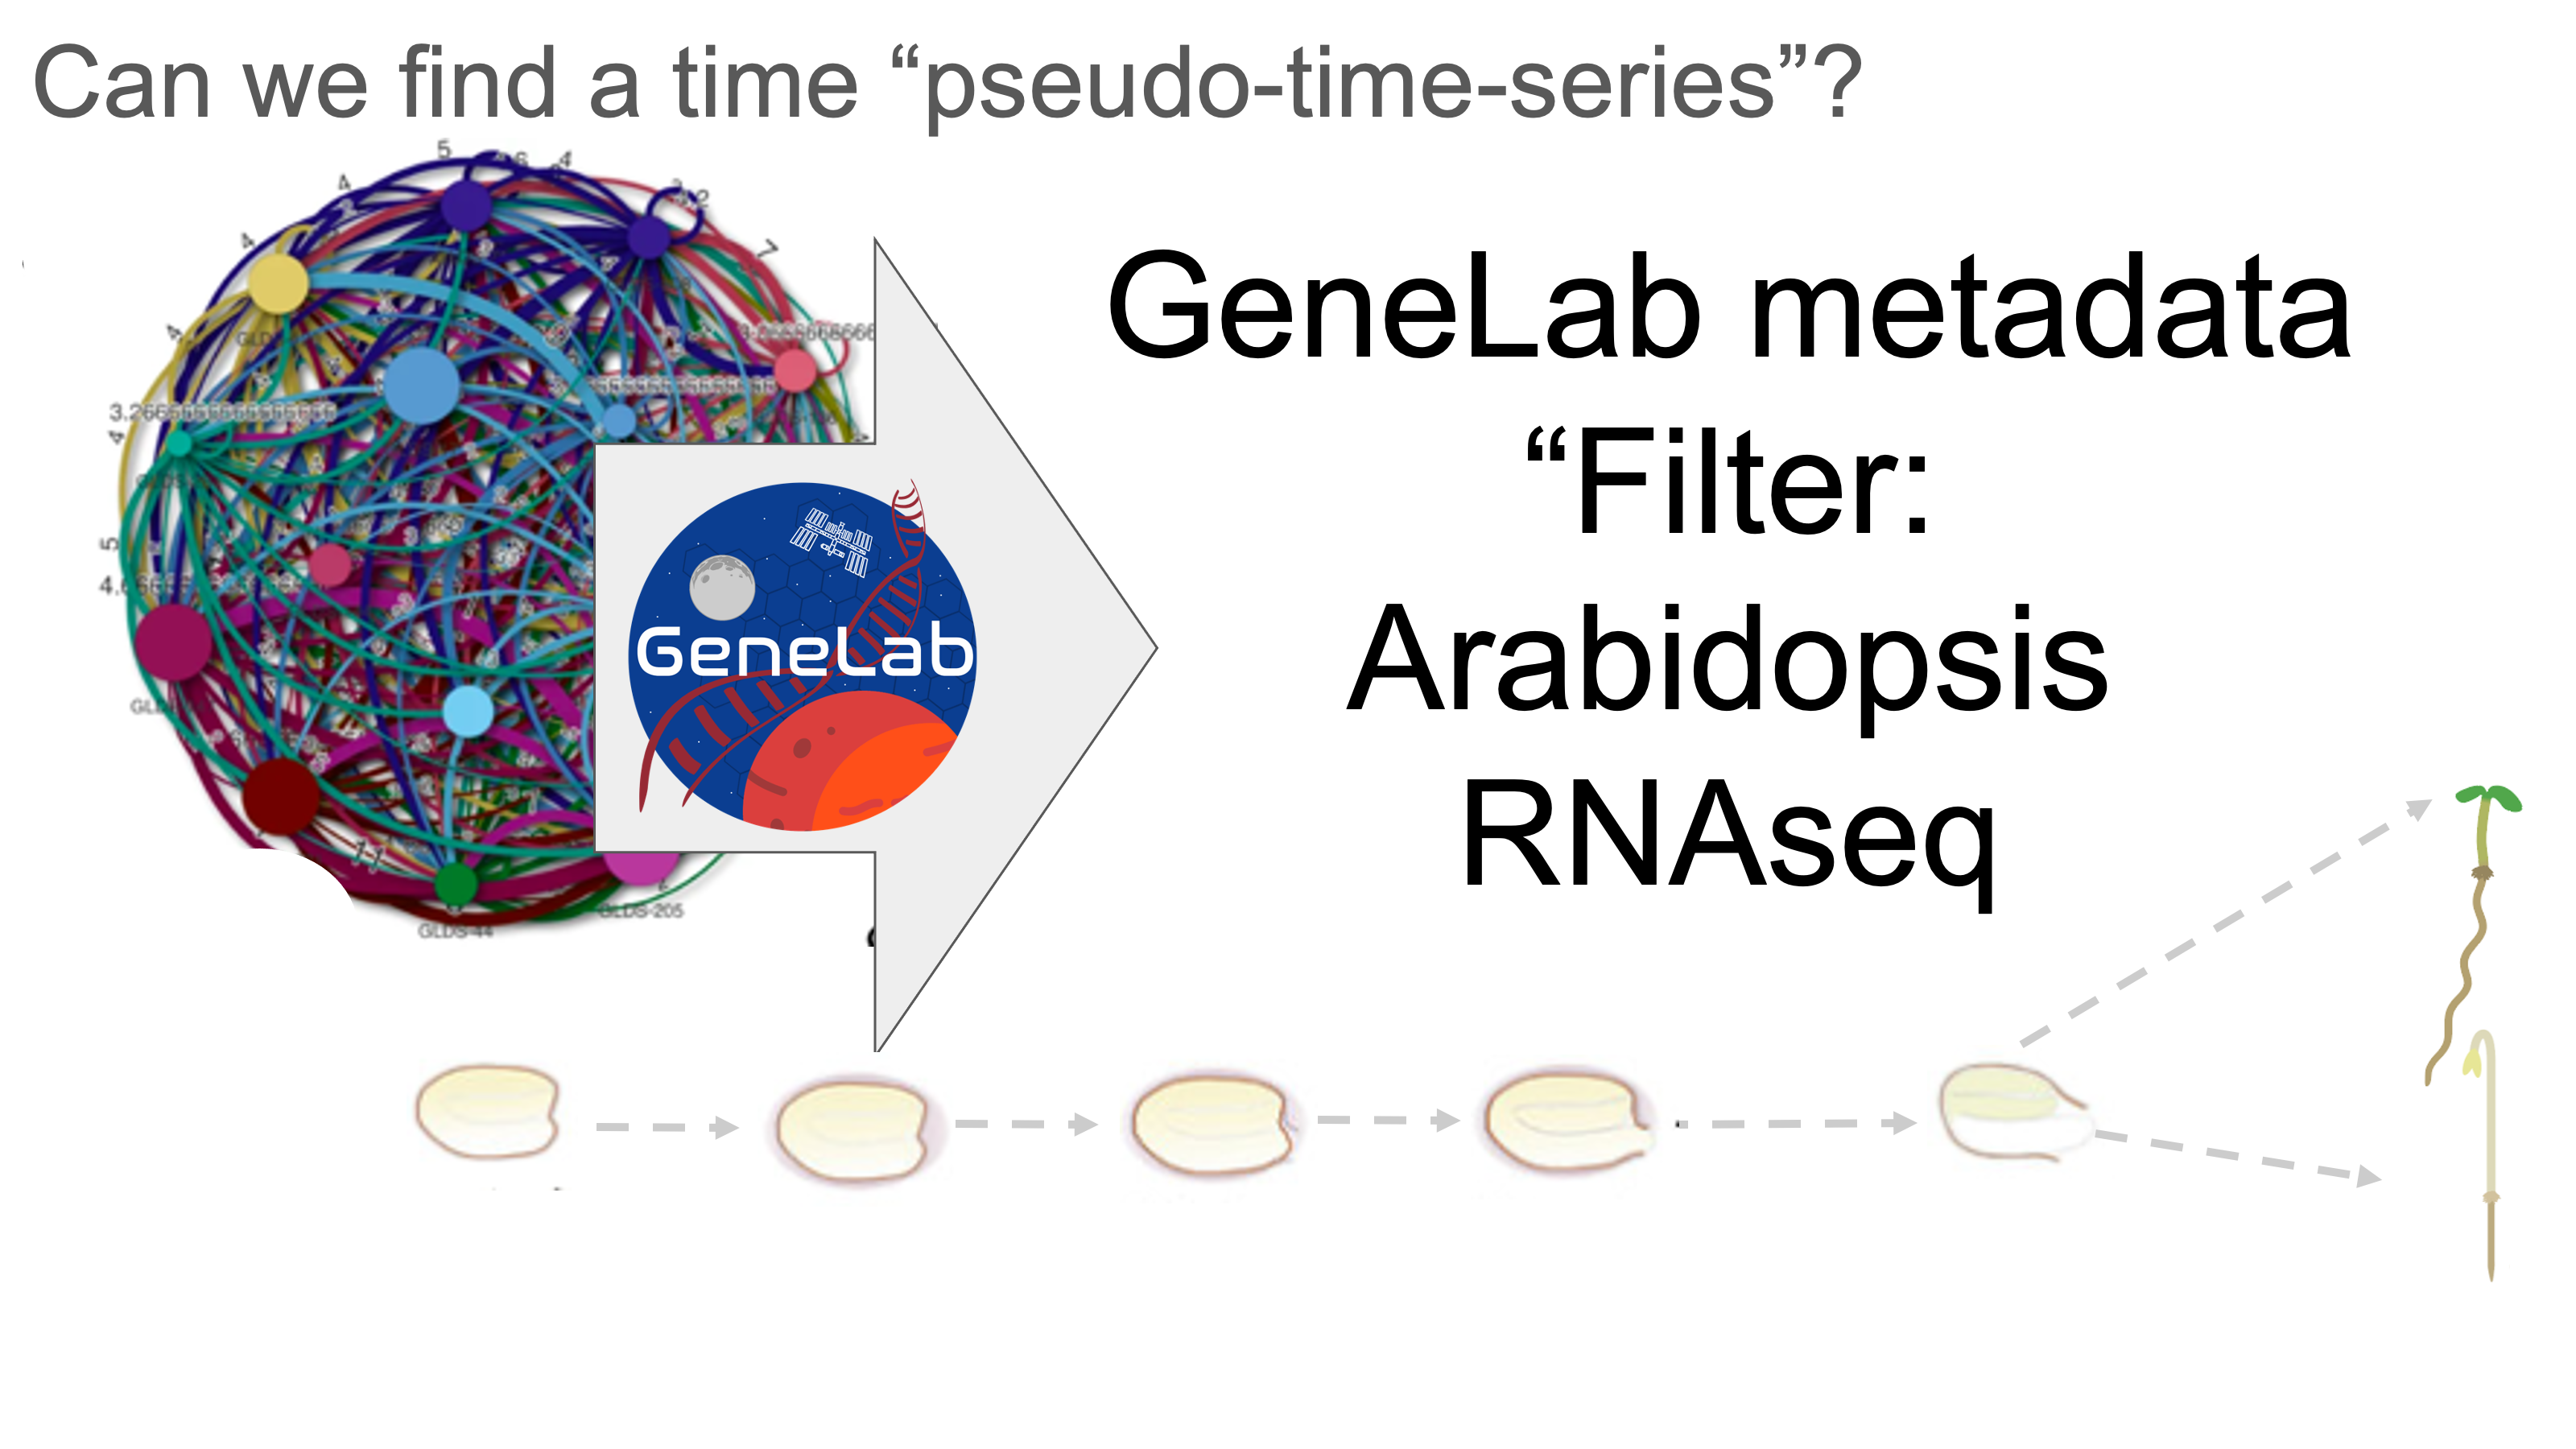
\includegraphics[width=0.85\textwidth]{figures/figure1_study_selection.png}
\caption{\textbf{Systematic selection and environmental parameterization of \textit{Arabidopsis} seedling spaceflight accessions.} Meta-analysis filtering strategy across NASA OSDR repository identifying datasets with overlapping biological replicates, dark/light regimes, and hardware enclosures (BRIC, APEX, EMCS) as described by \citet{barker2023meta}.}
\label{fig:study_selection}
\end{figure*}

\subsection{Pervasive Dominance of \textit{Ralstonia pickettii} in BRIC-19 (OSD-37)}
Taxonomic profiling of 8-day-old etiolated seedlings from the BRIC-19 mission (OSD-37) revealed a consistent microbial consortium across both spaceflight (FL) and ground control (GC) samples (Table~\ref{tab:taxa}). Strikingly, the betaproteobacterium \textit{Ralstonia pickettii} emerged as the overwhelmingly dominant taxon across all biological replicates and ecotypes. In the Cape Verde Islands (Cvi-0) accession, \textit{R. pickettii} accounted for 100\% of all classified microbial reads in multiple samples. In Columbia-0 (Col-0), Wassilewskija-2 (WS-2), and Landsberg \textit{erecta}-0 (Ler-0), \textit{R. pickettii} consistently constituted $>65\%$ of relative abundance.

Beyond \textit{R. pickettii}, OSD-37 libraries contained secondary populations of recognized plant-associated endophytes, including \textit{Herbaspirillum huttiense}, \textit{Pseudomonas fluorescens}, \textit{Curvibacter gracilis}, \textit{Acidovorax temperans}, and \textit{Agrobacterium tumefaciens}. While the primary community composition was conserved between orbit and ground, flight samples exhibited reproducible shifts in the relative abundance of secondary Proteobacteria, suggesting subtle microgravity-mediated or enclosure-induced alterations in host colonization.

\begin{figure*}[t]
\centering
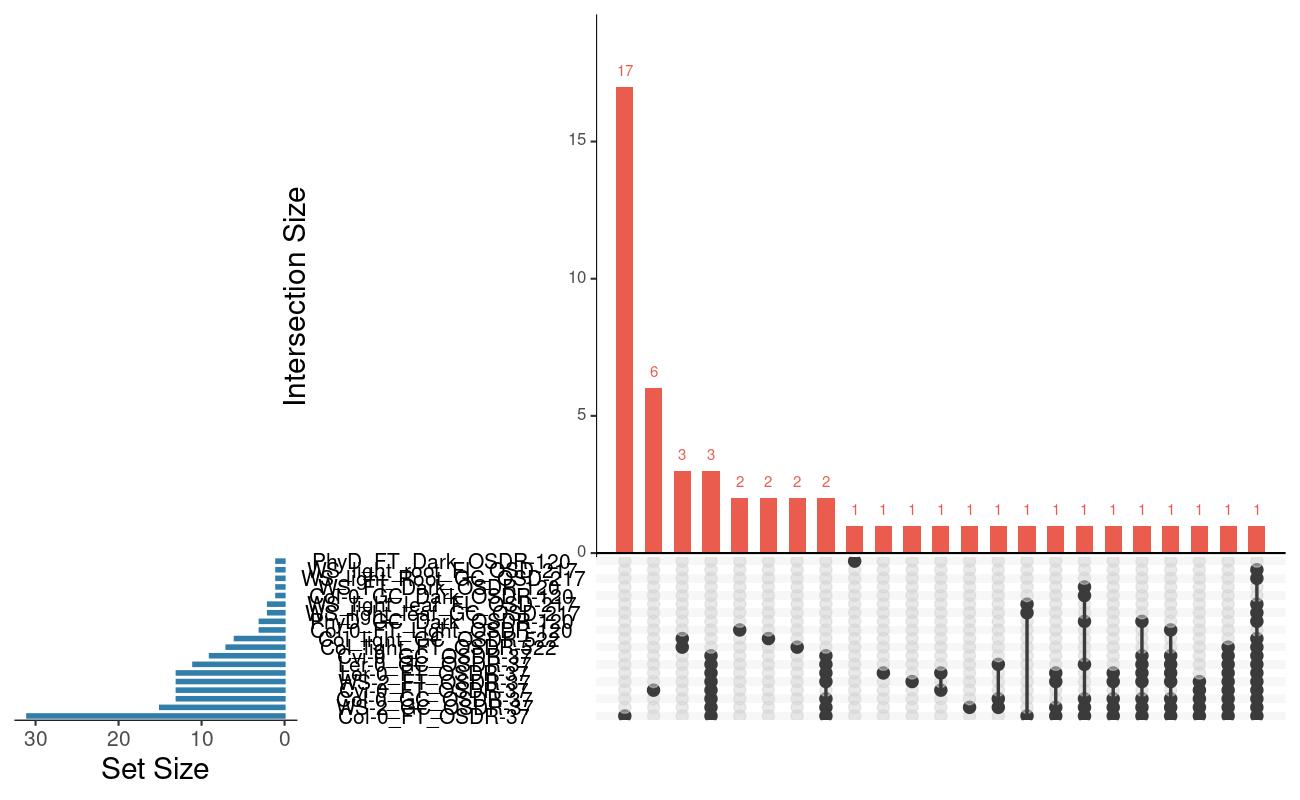
\includegraphics[width=0.92\textwidth]{figures/figure2_upset_plot.png}
\caption{\textbf{UpSet intersection of detected microbial taxa across spaceflight and ground seedling conditions.} Intersections demonstrate a shared core of seed-borne Proteobacteria (including \textit{Ralstonia pickettii} and \textit{Pseudomonas fluorescens}) alongside sample-specific environmental transfers and ecotype-restricted colonizers.}
\label{fig:upset}
\end{figure*}

\subsection{Discovery of \textit{Weizmannia ginsengihumi} in BRIC-20 (OSD-38)}
Analysis of younger 3--4-day-old Col-0 seedlings from BRIC-20 (OSD-38) uncovered a distinctly different microbial profile from the 8-day-old BRIC-19 seedlings. In the Ames Research Center ground control samples preserved via liquid nitrogen fixation (\path{GLDS-38_rna_seq_Atha_WT-Col-0_sl_LN2_Rep1_n2-1}), we identified the firmicute \textit{Weizmannia ginsengihumi} (formerly classified as \textit{Bacillus ginsengihumi}). 

This bacterium, renowned for producing active antioxidants and promoting growth in \textit{Panax ginseng}, had never previously been documented within spaceflight plant tissues or orbital cultivation hardware. Its detection in early germination stages suggests that \textit{W. ginsengihumi} exists as a quiescent seed endophyte that activates upon hydration and imbibition, potentially conferring oxidative stress resilience to the emerging seedling radicle.

\begin{figure*}[t]
\centering
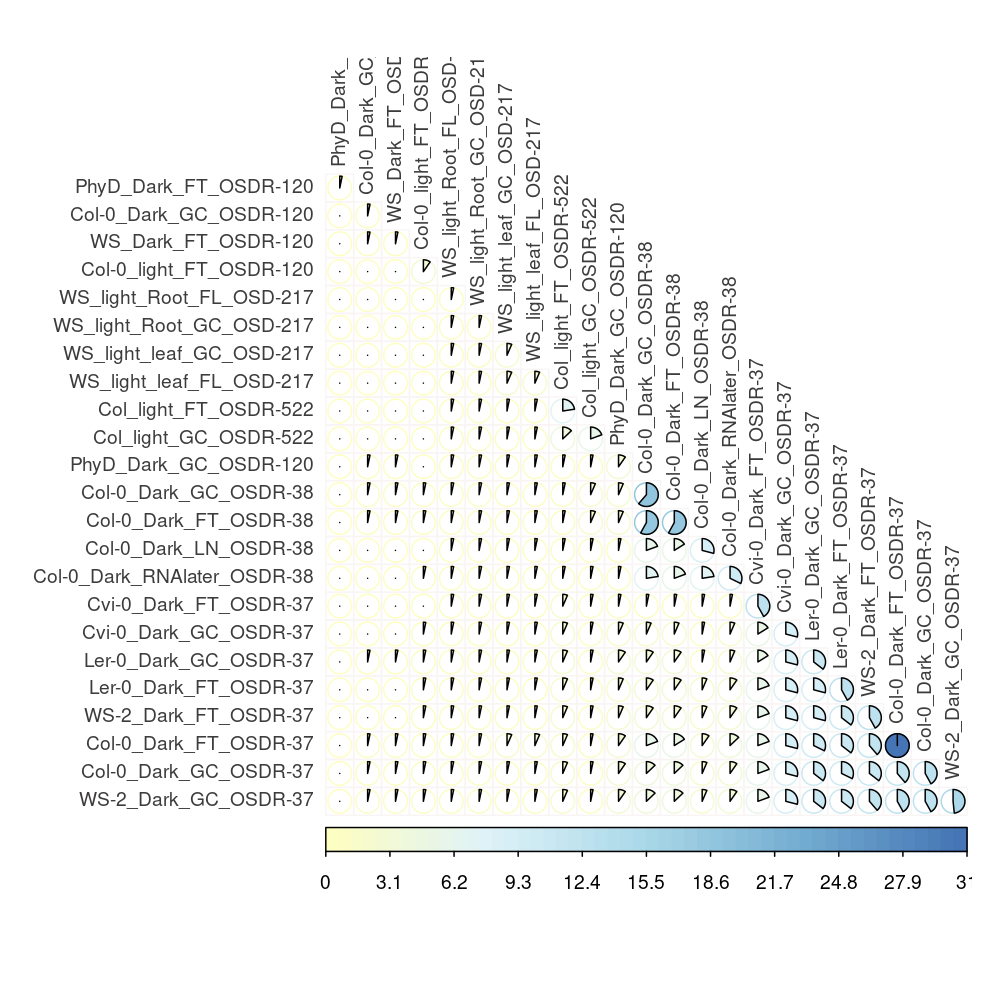
\includegraphics[width=0.88\textwidth]{figures/figure3_correlation_heatmap.png}
\caption{\textbf{Pairwise correlation heatmap of microbial community profiles.} Spearman correlation and hierarchical clustering of microbial profiles across experimental accessions, revealing clustering by mission hardware and plant developmental stage rather than flight status alone.}
\label{fig:heatmap}
\end{figure*}

\subsection{Tissue Partitioning and Microbial Depletion in Root Tips (OSD-120)}
A pivotal question in plant microbiome dynamics is whether endophytes universally colonize all vegetative organs or localize to specific anatomical zones. Analysis of APEX-03-2 (OSD-120), in which 11--13-day-old Col-0 and WS seedlings were grown under directional light regimes and micro-dissected specifically for root tips (apical meristem and elongation zones), produced a dramatic negative result: MetaPhlAn4 profiling reported an absence of detectable microbial taxa across both flight and ground replicates (\path{GLDS-120_rna_seq_Atha_Col-0_root_GC_dark_Rep3} and \path{WS_root_GC_dark_Rep3}).

This finding contrasts sharply with the whole-seedling data from OSD-37, OSD-38, and OSD-522, and with the separated leaf and root tissues of OSD-217. In OSD-217, leaf mesophyll and mature root vasculature harbored robust populations of \textit{Cutibacterium acnes}, \textit{Bradyrhizobium viridifuturi}, and \textit{Delftia acidovorans}. The stark absence of reads in OSD-120 confirms that the active root apical meristem is maintained in a nearly sterile state, while endophytic and epiphytic colonization is compartmentalized in differentiated hypocotyls, cotyledons, and mature vascular bundles.

\begin{figure}[t]
\centering
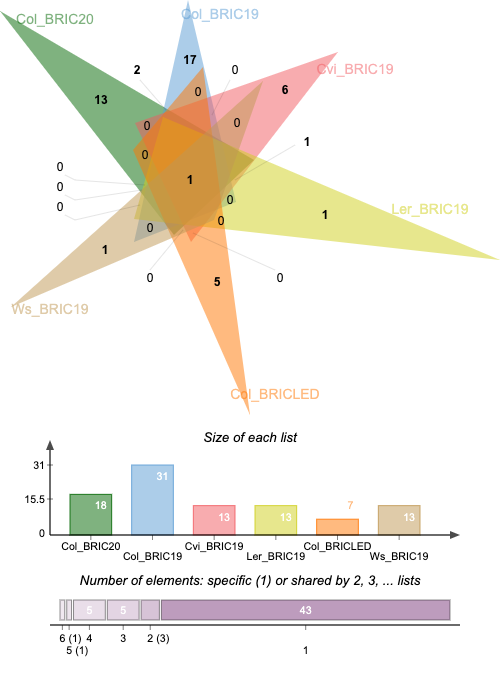
\includegraphics[width=0.48\textwidth]{figures/figure4_venn_chart.png}
\caption{\textbf{jVenn distribution of core seedling microbial associates.} Overlap between major flight experimental cohorts illustrating core persisting taxa versus transient mission-specific contaminants.}
\label{fig:venn}
\end{figure}

\subsection{Partitioning Intrinsic Endophytes from Human and Hardware Commensals}
By cross-referencing all detected taxa against The Microbe Directory and BacDive databases, we categorized the spaceflight seedling metatranscriptome into two distinct ecological guilds (Table~\ref{tab:taxa}):
\begin{enumerate}
    \item \textbf{Seed-Borne Plant Endophytes:} Dominated by environmental Proteobacteria and Firmicutes (\textit{Ralstonia pickettii}, \textit{Pseudomonas fluorescens}, \textit{Herbaspirillum huttiense}, \textit{Agrobacterium tumefaciens}, \textit{Weizmannia ginsengihumi}, \textit{Acidovorax temperans}, and \textit{Paenibacillus} spp.). These taxa were conserved across multiple independent laboratories and mission years, reflecting true internal seed transmission.
    \item \textbf{Human and Hardware Commensals:} Represented by classic human skin and mucosal colonizers, notably \textit{Cutibacterium acnes} (formerly \textit{Propionibacterium acnes}), \textit{Malassezia restricta} (an anthropophilic skin fungus), \textit{Corynebacterium aurimucosum}, \textit{Staphylococcus epidermidis}, and \textit{Escherichia coli}.
\end{enumerate}

These anthropophilic species were recovered consistently from flight hardware (BRIC canisters and Petri plate surfaces), providing direct molecular evidence of payload touch-transfer during pre-flight seed mounting, dish integration, or post-flight harvest on the ISS.


\section{Discussion}
\label{sec:discussion}

The exploration of plant microbiomes within extraterrestrial habitats represents a vital frontier for space agricultural research \citep{fu2016how}. Traditional spaceflight plant research has predominantly viewed seedlings through a reductionist lens, attributing physiological deviations solely to direct host cellular responses to microgravity and cosmic radiation \citep{paul2017genetic,choi2019variation}. By mining the non-host metatranscriptome from archival NASA OSDR accessions, this study provides compelling proof-of-concept that \textit{Arabidopsis} seedlings in space host complex, dynamic microbial consortia that cannot be ignored when evaluating spaceflight plant adaptation.

\subsection{The Seed as a Vehicle for Microbial Transfer to Space}
Standard spaceflight protocols mandate rigorous surface-sterilization of seeds using hypochlorite or ethanol solutions prior to plating \citep{dixit2021persistence}. The widespread survival and metabolic transcription of taxa like \textit{Ralstonia pickettii}, \textit{Pseudomonas fluorescens}, \textit{Herbaspirillum huttiense}, and \textit{Weizmannia ginsengihumi} confirm that surface chemical treatments fail to eliminate endophytic bacteria residing within the seed coat, aleurone layer, or embryo tissues.

This has profound implications for planetary protection and space farm biosecurity. As demonstrated by the persistent dominance of \textit{R. pickettii} across OSD-37 (up to 100\% in Cvi-0), single oligotrophic generalists can monopolize the seedling microbiome within closed containment hardware like the BRIC canisters. \textit{R. pickettii} is capable of surviving in extreme nutrient-depleted conditions, forming robust biofilms, and tolerating toxic metals and disinfectants \citep{segata2012metagenomic}. In microgravity, where fluid convection is absent and boundary-layer gas exchange is severely hindered, biofilm-forming bacteria could either exacerbate anoxic root-zone stress or, conversely, create localized microenvironments that buffer the plant against oxidative shock \citep{barker2023meta}.

\subsection{Discovery of \textit{Weizmannia ginsengihumi}: A Candidate Spaceflight Probiotic}
The detection of \textit{Weizmannia ginsengihumi} in OSD-38 highlights the power of archival metatranscriptome mining for bio-prospecting. In terrestrial agro-ecosystems, \textit{W. ginsengihumi} enhances host antioxidant defenses, synthesizes ginsenoside-modifying enzymes, and stimulates root elongation under abiotic stress \citep{kim2020weizmannia}. Given that plants in spaceflight chronically upregulate reactive oxygen species (ROS) scavengers, peroxidases, and oxidative stress pathways \citep{choi2019variation,kruse2020spaceflight}, the presence of an endophyte with intrinsic antioxidant-producing capabilities could represent a natural symbiotic adaptation. Future experiments should test whether intentional inoculation of crop seeds with \textit{W. ginsengihumi} or \textit{P. fluorescens} confers enhanced vigor, root architecture, and pathogen defense in orbital and lunar growth chambers.

\subsection{Human-Associated Commensals and Habitat Biosecurity}
The recurrent recovery of human skin commensals (\textit{Cutibacterium acnes}, \textit{Malassezia restricta}) and opportunistic bacteria (\textit{Escherichia coli}, \textit{Moraxella osloensis}) across OSD-37, OSD-120, and OSD-217 exposes the permeability of spaceflight hardware to crew microbiomes. Recent investigations by \citet{totsline2023microgravity,totsline2024simulated} demonstrated that microgravity induces wide stomatal opening while suppressing plant pattern-triggered immunity (PTI), facilitating stomatal ingression and internalization of human pathogens like \textit{Salmonella enterica} and \textit{E. coli} in salad crops. Our detection of active \textit{E. coli} and skin commensal transcripts in orbital plant RNA emphasizes the urgent need for stringent touch-transfer controls and microbiome monitoring in future crewed food production systems.

\subsection{Methodological Strengths and Limitations}
Extracting microbial signals from host RNA-seq data offers an exceptional, zero-mass, retroactive approach to space biology. Thousands of archival samples across OSDR and international repositories can be re-interrogated without necessitating new spaceflight missions. Nonetheless, several caveats must be considered:
\begin{enumerate}
    \item \textbf{Sequencing Library Bias:} Most OSDR plant RNA-seq libraries utilize poly(A) enrichment, which selectively enriches for eukaryotic mRNA. Non-polyadenylated bacterial transcripts are captured only through non-specific priming, partial polyadenylation during degradation, or co-purification. Consequently, relative read counts reflect a mixture of absolute abundance and transcriptional turnover.
    \item \textbf{Low Biomass Artifacts:} When host tissue biomass is minuscule—as in the micro-dissected root tips of OSD-120—the ratio of microbial reads to background noise drops below detection thresholds, as observed here.
    \item \textbf{Cross-Study Heterogeneity:} Differences in RNA preservation reagents (RNAlater vs.\ liquid nitrogen) significantly alter microbial RNA degradation kinetics \citep{kruse2017transcriptome}.
\end{enumerate}

To overcome these limitations, future spaceflight multi-omics initiatives should systematically incorporate dual RNA-seq protocols (total RNA extraction with concurrent ribosomal RNA depletion of both plant and microbial rRNAs), coupled with long-read metagenomic sequencing on orbit via MinION or Oxford Nanopore sequencers.


\section{Declarations}
\label{sec:declarations}

\subsection{Acknowledgements}
The authors acknowledge the NASA GeneLab and Open Science Data Repository (OSDR) teams for curating, maintaining, and providing open access to spaceflight omics datasets. We also thank the members of the NASA GeneLab Plant Analysis Working Group (AWG) for insightful discussions regarding spaceflight hardware, metadata harmonization, and seedling biology.

\subsection{Author Contributions}
R.J.B. and Z.S. conceived and designed the study. Z.S. executed the bioinformatic data extraction, MetaPhlAn4 profiling, UpSetR, and correlation analyses. R.J.B. supervised the research, conducted biological interpretation, and drafted the manuscript. All authors reviewed, edited, and approved the final version of the manuscript.

\subsection{Funding}
This work was supported by the AstroBotany Artificial Intelligence Research Initiative (AIRI) and related NASA space biology research grants.

\subsection{Conflict of Interest}
The authors declare no competing financial or non-financial interests.

\subsection{Data Availability}
All raw sequencing datasets and metadata analyzed in this manuscript are publicly available from the NASA Open Science Data Repository (OSDR, \url{https://osdr.nasa.gov}) under accession numbers OSD-37 (GLDS-37), OSD-38 (GLDS-38), OSD-120 (GLDS-120), OSD-217 (GLDS-217), OSD-321 (GLDS-321), and OSD-522 (GLDS-522).

\subsection{Code Availability}
The bioinformatic workflows, automated FASTQ download scripts, Google Colab notebooks, and analysis code are openly accessible on GitHub at: \\
\url{https://github.com/dr-richard-barker/Microbiome_of_seedlings_in_space}.


% --- Bibliography ---
\bibliographystyle{plainnat}
\bibliography{references}

\end{document}
